\documentclass{beamer}

\usepackage{epsfig}
\usepackage{multicol}
\usepackage{geometry}
%\usepackage[dvipsnames]{xcolor}
\usepackage{textcomp}
\usepackage{graphicx}
\usepackage{caption}
\usepackage{subcaption}
\usepackage{amsmath}
\usepackage{tcolorbox}
\usetheme{Boadilla}
\usepackage{pict2e}
\usepackage{tikz}
\usepackage{xcolor}

\title[Traitement du signal numérique]{Traitement du signal numérique - HEI4 IMS}
\author[Antony Bazir]{}

\setlength{\unitlength}{1cm}

\begin{document}
\section{Rappel}
\begin{frame}
\frametitle{Rappels : Signaux }
\textbf{Signal numérique =  codage + échantillonnage}
\begin{center}
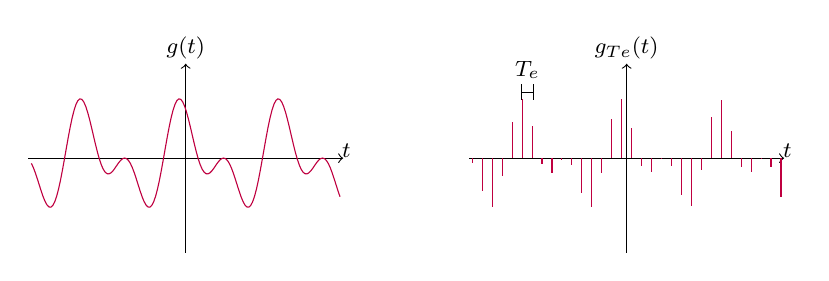
\begin{tikzpicture}
\begin{scope}[scale=0.4]
	\draw[->] (-5,0)-- (5,0);
%\draw (-0.3,-0.3) node {0};
\draw[->] (0,-3)-- (0,3);
\draw (5.1,0.25) node {\footnotesize{$t$}};
\draw (0,3.5) node {\footnotesize{$g(t)$}};
%\draw (4.5,-0.3) node {1};

\draw[domain=-4.9:4.9,color=purple,samples=160] plot (\x,{2*(0.55*cos(2*\x r)+ 0.45*cos(2*2*(\x+3.14/12) r))});
\end{scope}

\begin{scope}[scale=0.4,xshift=14cm]
	\draw[->] (-5,0)-- (5,0);
%\draw (-0.3,-0.3) node {0};
\draw[->] (0,-3)-- (0,3);
\draw (5.1,0.25) node {\footnotesize{$t$}};
\draw (0,3.5) node {\footnotesize{$g_{Te}(t)$}};
%\draw (4.5,-0.3) node {1};
\draw[|-|] (-2.95,2.1)--(-3.35,2.1);
\draw (-3.15,2.8) node {\footnotesize{$T_e$}};

\draw[domain=-4.9:4.9,color=purple,samples=32] plot[ycomb] (\x,{2*(0.55*cos(2*\x r)+ 0.45*cos(2*2*(\x+3.14/12) r))});
%\draw[domain=-4.9:4.9,dotted,color=purple,samples=32] plot[xcomb] (\x,{2*(0.55*cos(2*\x r)+ 0.45*cos(2*2*(\x+3.14/12) r))});
\end{scope}
	\end{tikzpicture}
\end{center}
\vspace{0.5cm}
\begin{itemize}
\item \'Echantillonage : discrétisation en temps
\vspace{0.3cm}
\item Codage : discrétisation en amplitude
\end{itemize}
\end{frame}

\begin{frame}
\frametitle{Rappel : Analyse de signaux}
Pour les signaux discrets on utilise TOUJOURS la transformée en Z
\[\boxed{TZ\{ f \}(z) = \sum_{n = -\infty}^{\infty} f[n] z^{-n}} \]
On en dérive la transformée de Fourier 
\[\boxed{TF\{ f \}(\nu) = \sum_{n = -\infty}^{\infty} f[n] e^{-j 2 \pi n \nu T_e}} \]
\vspace{0.2cm}
La transformée de Fourier donne ce qu'on appelle le \textbf{spectre fréquentiel/réponse en fréquence} d'un signal/système
\end{frame}

\begin{frame}
\frametitle{Rappel : Analyse de signaux}
Les spectres fréquentiels/réponses en fréquences sont \textbf{généralement complexes}
\begin{center}
\begin{tikzpicture}
\begin{scope}[scale=0.4]
	\draw[->] (-5,0)-- (5,0);
%\draw (-0.3,-0.3) node {0};
\draw[->] (0,-3)-- (0,3);
\draw (5.1,0.25) node {\footnotesize{$t$}};
\draw (0,3.5) node {\footnotesize{$g_{Te}(t)$}};
%\draw (4.5,-0.3) node {1};
\draw[|-|] (-2.95,2.1)--(-3.35,2.1);
\draw (-3.15,2.8) node {\footnotesize{$T_e$}};

\draw[domain=-4.9:4.9,color=purple,samples=32] plot[ycomb] (\x,{2*(0.55*cos(2*\x r)+ 0.45*cos(2*2*(\x+3.14/12) r))});
%\draw[domain=-4.9:4.9,dotted,color=purple,samples=32] plot[xcomb] (\x,{2*(0.55*cos(2*\x r)+ 0.45*cos(2*2*(\x+3.14/12) r))});
\end{scope}
	\end{tikzpicture}
\end{center}

\begin{columns}
\column{60mm}
\underline{\small{Réponse en amplitude (Module  TF)}}:\\
\begin{center}
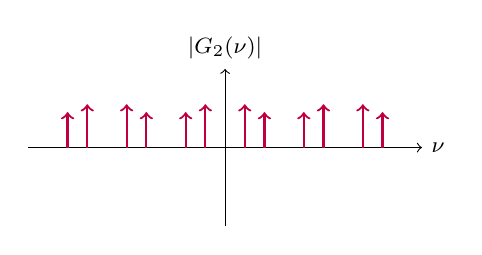
\begin{tikzpicture}
\begin{scope}
\draw[->] (-2.5,0)--(2.5,0) node[right]{\footnotesize{$\nu$}};
\draw[->] (0,-1)--(0,1) node[above]{\footnotesize{$|G_2(\nu)|$}};
\draw[->,purple,thick] (-1/4,0)--(-1/4,0.55) ;
\draw[->,purple,thick] (1/4,0)--(1/4,0.55) ;
\draw[->,purple,thick] (-2/4,0)--(-2/4,0.45) ;
\draw[->,purple,thick] (2/4,0)--(2/4,0.45) ;

\draw[->,purple,thick] (-1/4+1.5,0)--(-1/4+1.5,0.55) ;
\draw[->,purple,thick] (1/4+1.5,0)--(1/4+1.5,0.55) ;
\draw[->,purple,thick] (-2/4+1.5,0)--(-2/4+1.5,0.45) ;
\draw[->,purple,thick] (2/4+1.5,0)--(2/4+1.5,0.45) ;

\draw[->,purple,thick] (-1/4-1.5,0)--(-1/4-1.5,0.55) ;
\draw[->,purple,thick] (1/4-1.5,0)--(1/4-1.5,0.55) ;
\draw[->,purple,thick] (-2/4-1.5,0)--(-2/4-1.5,0.45) ;
\draw[->,purple,thick] (2/4-1.5,0)--(2/4-1.5,0.45) ;
\end{scope}
\end{tikzpicture}
\end{center}


\column{60mm}
\underline{\small{Réponse en phase (Argument TF)}}:\\
\begin{center}
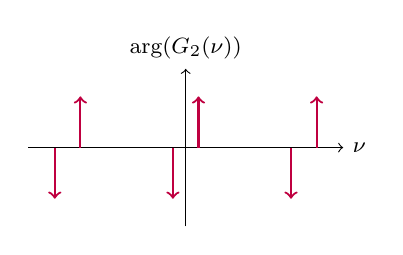
\begin{tikzpicture}
\begin{scope}
\draw[->] (-2,0)--(2,0) node[right]{\footnotesize{$\nu$}};
\draw[->] (0,-1)--(0,1) node[above]{\footnotesize{$\text{arg}(G_2(\nu))$}};
\draw[->,purple,thick] (-0.65/4,0)--(-0.65/4,-0.65) ;
\draw[->,purple,thick] (0.65/4,0)--(0.65/4,0.65) ;

\draw[->,purple,thick] (-0.65/4-1.5,0)--(-0.65/4-1.5,-0.65) ;
\draw[->,purple,thick] (0.65/4-1.5,0)--(0.65/4-1.5,0.65) ;

\draw[->,purple,thick] (-0.65/4+1.5,0)--(-0.65/4+1.5,-0.65) ;
\draw[->,purple,thick] (0.65/4+1.5,0)--(0.65/4+1.5,0.65) ;

\end{scope}
\end{tikzpicture}
\end{center}
\end{columns}

\end{frame}

\begin{frame}
\frametitle{TFD}
\[TF\{ x \}(\nu) = \sum_{n = -\infty}^{\infty} x[n] e^{-j 2 \pi n \nu T_e} \]
La transformée de Fourier d'un signal discret n'est pas calculables par un ordinateur...\\
\vspace{0.6cm}
Transformée de Fourier \textbf{Discrète}
\[ TFD\{ x \}[m] = \frac{1}{N} \sum_{n = 0}^{N-1} x[n] \; e^{-j 2 \pi n \frac{m}{N}}  \] 
\vspace{0.3cm}
Approximation de la transformée de Fourier...
\end{frame}

\begin{frame}
\frametitle{TFD}
Transformée de Fourier Discrète (TFD) $=$ Approximation du spectre sur $N$ points
\begin{columns}
\column{60mm}
\begin{center}
\begin{tikzpicture}
\begin{scope}[scale=0.4]
\draw[->] (-5,0)-- (5,0);
\draw[->] (0,-3)-- (0,3);
\draw (5.1,0.25) node {\footnotesize{$t$}};
\draw (0,3.5) node {\footnotesize{$g_{Te}(t)$}};
%\draw (4.5,-0.3) node {1};
\draw[|-|] (-2.95,2.1)--(-3.35,2.1);
\draw (-3.15,2.8) node {\footnotesize{$T_e$}};

\draw[domain=-4.9:4.9,color=purple,samples=32] plot[ycomb] (\x,{2*(0.55*cos(2*\x r)+ 0.45*cos(2*2*(\x+3.14/12) r))});
%\draw[domain=-4.9:4.9,dotted,color=purple,samples=32] plot[xcomb] (\x,{2*(0.55*cos(2*\x r)+ 0.45*cos(2*2*(\x+3.14/12) r))});
\end{scope}
\end{tikzpicture}\\
\footnotesize{\textit{Signal numérisée}}
\end{center}
\column{60mm}
\begin{center}
\begin{tikzpicture}
\begin{scope}[scale=0.4]
\draw[->] (0,0)-- (7,0);
\draw[->] (0,0)-- (0,6);
\draw (7.3,0.25) node {\footnotesize{$m$}};
\draw (0,6.5) node {\footnotesize{$TFD$}};
\draw[thick,purple] plot file {tfd_2cos.txt};
\end{scope}
\end{tikzpicture}\\
\footnotesize{\textit{TFD obtenue en Matlab (amplitude)}}
\end{center}
\end{columns}
Note: Si on rajoute des zéros à la fin du signal on interpole le spectre. (zero-padding)
\end{frame}

%\draw[thick,blue] plot file {module_freq_samp.txt};

\section{Détection complexe QRS}
\begin{frame}
\frametitle{Filtrage numérique :  Extraction du complexe QRS}
\begin{center}
\includegraphics[scale=0.35]{tr_num_ecg.png}\\
\textit{\footnotesize Algorithme de détection du complexe QRS, Tompkins, 2000}\\
\end{center}
Filtrage temps réel du signal numérique \& Extraction du complexe QRS\\
\vspace{0.3cm}
Pourquoi extraire le complexe QRS ?\\
\vspace{0.2cm}
\begin{itemize}
\item suivi de la condition du patient en temps réel 
\item Etablissement des tachogrammes (RR)
\item \'A la base de beacoup d'algorithmes acutels...
\end{itemize}

\end{frame}

\begin{frame}
\frametitle{Filtrage numérique :  Extraction du complexe QRS}
\textbf{Caractéristiques du complexe QRS}
\begin{center}
\includegraphics[scale=0.35]{QRS.png}\\

\end{center}
\underline{Origine physique} : dépolarisation des ventricules\\
\vspace{0.3cm}
Caractéristiques: \\
\vspace{0.1cm}
\begin{itemize}
\item Durée :  80 -100 ms
\item Fréquence : 10-15 Hz 
\end{itemize}

\end{frame}

\subsection{Filtrage passe-bande}
\begin{frame}
\frametitle{Filtrage numérique :  Extraction du complexe QRS}
\begin{center}
\includegraphics[scale=0.3]{ECG_spectrum.png}\\
\textit{\scriptsize Spectre en amplitude de l'ECG, Tompkins,2000}\\
\vspace{0.1cm}
\end{center}
Importance du filtrage passe-bande...
\end{frame}

\begin{frame}
\frametitle{Filtrage numérique :  Extraction du complexe QRS}
\begin{center}
\includegraphics[scale=0.3]{ECG_spectrum.png}\\
\textit{\scriptsize Spectre en amplitude de l'ECG, Tompkins,2000}\\
\vspace{0.1cm}
\end{center}
Comment choisir $T_e$ ? \only<2-> {Shannon $\rightarrow \nu_e > 80 Hz$  \only<3->{ Dans les faits, $\nu_e = $ 500 Hz} }


\end{frame}

\begin{frame}
\frametitle{Détection QRS: Filtrage passe-bande}
\begin{center}
\includegraphics[scale=0.35]{tr_num_ecg.png}\\
\textit{\footnotesize Algorithme de détection du complexe QRS, Tompkins, 2000}\\
\vspace{0.3cm}
\end{center}
Filtrage temps réel du signal numérique \& Extraction du QRS
\begin{enumerate}
\item \textbf{filtrage passe-bande numérique}
\item Dérivée 
\item Mise au carré 
\item Moyennage
\end{enumerate}
\end{frame}

\begin{frame}
\frametitle{Détection QRS: Filtrage passe-bande}
 \textbf{Filtrage passe-bande numérique}\\
 \vspace{0.3 cm}
 Plusieurs méthodes possibles (liste non-exhasutive) :\\
 \vspace{0.2cm}
 \begin{itemize}
 \item Filtre récursif à  2 pôles
 \vspace{0.2cm}
 \item Filtre à coefficients "entiers"
 \vspace{0.2cm}
 \end{itemize}
\end{frame}

\begin{frame}
\frametitle{Détection QRS: Filtrage passe-bande}
 \textbf{Filtrage passe-bande numérique: Filtre récursif à  2 pôles}\\
 \vspace{0.3 cm}
 Forme possible de la fonction de transfert :
 \[H(z) = \frac{c_1}{z-p_1} + \frac{c_2}{z-p_2} \]\\
  \vspace{0.3 cm}
\only<2->{
  Tout filtre récursif analogique peut se décomposer sous la forme 
\[ H(s)  =  \frac{(s-z_1)(s-z_2)...(s-z_n)}{(s-p_1)(s-p_2)...(s-p_n)} = \frac{c_1}{s-p_1} + \frac{c_2}{s-p_2} + \cdots + \frac{c_n}{s-p_n} \] 
}
\only<3>{
Cela permet de construire des filtres numériques avec les bonnes propriétés à partir de sous-unités de forme  $\frac{\displaystyle c_k}{ \displaystyle 1-e^{p_k T_e}z^{-1}}$ (Invariance impulsionnelle)
}  
\end{frame}



\begin{frame}
\frametitle{Détection QRS: Filtrage passe-bande}
 \textbf{Filtrage passe-bande numérique: Filtre récursif à  2 pôles}\\
 \vspace{0.3 cm}
 Forme possible de la fonction de transfert :
 \[H(z) = \frac{c_1}{z-p_1} + \frac{c_2}{z-p_2} \]\\
  \vspace{0.3 cm}
  \'Equation aux différences :
 \[y[n] = b_1 y[n-1] - b_2 y[n-2] + x[n] - x[n-2] \]  
\end{frame}

\begin{frame}
\frametitle{Détection QRS: Filtrage passe-bande}
 \textbf{Filtrage passe-bande numérique: Filtre récursif à  2 pôles}\\

  Forme de l'équation aux différences :
 \[y[n] = b_1 y[n-1] - b_2 y[n-2] + x[n] - x[n-2] \]  \\
  \vspace{0.3 cm}
  Fonction de transfert :
   \[H(z) = \frac{1 - z^{-2}}{1 - b_1 z^{-1} + b_2 z^{-2}} \]  \\
  \vspace{0.3cm}
 \textbf{Comment se comporte ce filtre ?}
\end{frame}

\begin{frame}
\frametitle{Détection QRS: Filtrage passe-bande}
 \textbf{Filtrage passe-bande numérique: Filtre récursif à  2 pôles}\\

  \vspace{0.3 cm}
  Fonction de transfert :
   \[H(z) = \frac{1 - z^{-2}}{1 - b_1 z^{-1} + b_2 z^{-2}} \]  \\
  \vspace{0.3cm}
 On prend les valeurs données par Tompkins:
 \begin{itemize}
 \item $f_e$ = 500 Hz
 \item $b_1$ = 1.875
 \item $b_2$ = 0.9219
 \end{itemize}
\end{frame}

\begin{frame}
\frametitle{Détection QRS: Filtrage passe-bande}
 \textbf{Filtrage passe-bande numérique: Filtre récursif à  2 pôles}\\

  \vspace{0.3 cm}
  Fonction de transfert :
   \[H(z) = \frac{1 - z^{-2}}{1 - 1.875 z^{-1} + 0.9219 z^{-2}} \]  \\
  \vspace{0.3cm}
   \[H(\nu) = \frac{1 - e^{-4 j \pi \frac{\nu}{500}}}{1 - 1.875 e^{-2 j \pi \frac{\nu}{500}} + 0.9219  e^{-4 j \pi \frac{\nu}{500}}} \] 

\end{frame}

\begin{frame}
\frametitle{Détection QRS: Filtrage passe-bande}
 \textbf{Filtrage passe-bande numérique: Filtre récursif à  2 pôles}\\
\[H(\nu) = \frac{1 - e^{-4 j \pi \frac{\nu}{500}}}{1 - 1.875 e^{-2 j \pi \frac{\nu}{500}} + 0.9219  e^{-4 j \pi \frac{\nu}{500}}} \] 
\begin{center}
\begin{tikzpicture}
\begin{scope}[scale=2.5]
\draw[->] (0,0)-- (1.1,0)node[right] {\scriptsize $\nu$} ;
\draw[->] (0,0)-- (0,1.2)node[above] {\scriptsize  $|H(\nu)|$};
\draw[thick,blue] plot file {module_passebande1.txt};

\draw[dashed] (0.07,0) node[below]{\scriptsize 17 Hz}--(0.07,1);
\draw[dashed] (1,0) node[below]{\scriptsize 250 Hz}--(1,0);
\end{scope}

\end{tikzpicture}
\end{center}
\vspace{0.3cm}
On sélectionne bien dans une gamme de fréquence autour du QRS (0-35 Hz)
\end{frame}

\begin{frame}
\frametitle{Détection QRS: Filtrage passe-bande}
 \textbf{Filtrage passe-bande numérique: Filtre récursif à  2 pôles}\\
\begin{columns}
\column{60mm}
\[H(\nu) = \frac{1 - e^{-4 j \pi \frac{\nu}{500}}}{1 - 1.875 e^{-2 j \pi \frac{\nu}{500}} + 0.9219  e^{-4 j \pi \frac{\nu}{500}}} \]
\column{60mm} 
\begin{center}
\begin{tikzpicture}
\begin{scope}[scale=2.5]
\draw[->] (0,0)-- (1.1,0)node[right] {\scriptsize $\nu$} ;
\draw[->] (0,0)-- (0,1.2)node[above] {\scriptsize  $|H(\nu)|$};
\draw[thick,blue] plot file {module_passebande1.txt};

\draw[dashed] (0.07,0) node[below]{\scriptsize 17 Hz}--(0.07,1);
\draw[dashed] (1,0) node[below]{\scriptsize 250 Hz}--(1,0);
\end{scope}

\end{tikzpicture}
\end{center}
\end{columns}
\vspace{0.3cm}
Remarques :
\begin{itemize}
\item Le numérateur sert à couper les basses fréquences
\item Coefficients optimisées pour augmenter la vitesse de calcul
\end{itemize}
\end{frame}

\begin{frame}
\frametitle{Détection QRS: Filtrage passe-bande}
 \textbf{Filtrage passe-bande numérique: Filtre récursif à  2 pôles}\\
\begin{columns}
\column{60mm}
\[H(\nu) = \frac{1 - e^{-4 j \pi \frac{\nu}{500}}}{1 - 1.875 e^{-2 j \pi \frac{\nu}{500}} + 0.9219  e^{-4 j \pi \frac{\nu}{500}}} \]
\column{60mm} 
\begin{center}
\begin{tikzpicture}
\begin{scope}[scale=2.5]
\draw[->] (0,0)-- (1.1,0)node[right] {\scriptsize $\nu$} ;
\draw[->] (0,-0.6)-- (0,0.6)node[above] {\scriptsize  $\text{arg}(H(\nu))$};
\draw[thick,blue] plot file {argument_passebande1.txt};

\draw[dashed] (0.07,0) node[below]{\scriptsize 17 Hz}--(0.07,0);
\draw[dashed] (1,0) node[below]{\scriptsize 250 Hz}--(1,0);
\end{scope}

\end{tikzpicture}
\end{center}
\end{columns}
Problèmes :
\begin{itemize}
\item Phase fortement non linéaire
\item Distorsion de phase importante au niveau de la bande d'intérêt
\end{itemize}
\only<2->{
On utilise un autre type de filtre...
}
\end{frame}

\begin{frame}
\frametitle{Détection QRS: Filtrage passe-bande}
 \[y[n] = b_1 y[n-1] - b_2 y[n-2] + x[n] - x[n-2] \]
\begin{columns}[T]
\column{60mm}
\begin{center}
\begin{tikzpicture}
\begin{scope}[scale=2]
\draw[->] (0,0)-- (2.1,0)node[right] {\scriptsize $n$} ;
\draw[->] (0,-0.6)-- (0,1.2)node[above] {\scriptsize  $x[n]$};
\draw[thick,blue] plot file {x_ecg_tompkins.txt};
\end{scope}
\end{tikzpicture}
\end{center}
\column{60mm}
\begin{center}
\begin{tikzpicture}
\begin{scope}[scale=2]
\draw[->] (0,0)-- (2.1,0)node[right] {\scriptsize $n$} ;
\draw[->] (0,-0.6)-- (0,1.2)node[above] {\scriptsize  $y[n]$};
\draw[thick,blue] plot file {ecg_tompkins.txt};
\end{scope}
\end{tikzpicture}
\end{center}
\begin{center}
\begin{tikzpicture}

\end{tikzpicture}
\end{center}
\end{columns}
\end{frame}

\begin{frame}
\frametitle{Détection QRS: Filtrage passe-bande}
 \textbf{Filtrage passe-bande numérique: Filtre à coeffs entiers}\\
 \vspace{0.2cm}
 \underline{Objectif} : Gagner du temps de calcul en prenant des coeffs entiers ET garder une phase linéaire (informatique) \\
 \vspace{0.3cm}
 Forme générale : 
 \[ H(z) = \frac{(1 -z^{-m})^p}{(1 - 2 \cos(\theta)z^{-1} + z^{-2})^t} \] \\
 \vspace{0.2cm}
 \begin{itemize}
 \item  $m$,$p$ et $t$ entiers positifs
 \item $\theta$ idéalement 0, $\pi/3$, $\pi/2$, $2\pi/3$ ou $\pi$
 \item Permet "d'annuler" des zéros
 \end{itemize}
\end{frame}

\begin{frame}
\frametitle{Détection QRS: Filtrage passe-bande}
 \textbf{Filtrage passe-bande numérique: Filtre à coeffs entiers}\\
 \vspace{0.2cm}
 Forme générale : 
 \[ H(z) = \frac{(1 -z^{-m})^p}{(1 - 2 \cos(\theta)z^{-1} + z^{-2})^t} \] \\
 \vspace{0.2cm}
 Mise en oeuvre pour la détection QRS :
 \begin{itemize}
 \item  Passe-haut et passe-bas en cascade
 \item \textbf{Phase linéaire} $\rightarrow$ pas de distorsion de phase
 \end{itemize}
 \vspace{0.2cm}
 \textbf{Important de ne pas trop déformer l'ECG pendant le traitement...}
\end{frame}

\begin{frame}
\frametitle{Détection QRS: Filtrage passe-bande}
 \textbf{Passe-bas à coeff entiers}\\
  \vspace{0.2cm}
   \[ H_{pb}(z) = \frac{(1 -z^{-6})^2}{(1 - z^{-1} )^2} \]
   \vspace{0.1cm}
   \begin{columns}
	\column{60mm}
	\begin{center}
	\begin{tikzpicture}
	\begin{scope}[scale=3]
\draw[->] (0,0)-- (1.1,0)node[right] {\scriptsize $\nu$} ;
\draw[->] (0,0)-- (0,1.2)node[above] {\scriptsize  $|H(\nu)|$};
\draw[thick,blue] plot file {module_passebas.txt};

\draw[dashed] (0.33,0) node[below]{\scriptsize 33 Hz}--(0.33,0);
\draw[dashed] (1,0) node[below]{\scriptsize 100 Hz}--(1,0);
	\end{scope}
	\end{tikzpicture}
	\end{center}
	\column{60mm}  
		\begin{center}
	\begin{tikzpicture}
	\begin{scope}[scale=3]
\draw[->] (0,0)-- (1.1,0)node[right] {\scriptsize $f$} ;
\draw[->] (0,-0.6)-- (0,0.6)node[above] {\scriptsize  $\text{arg}(H(f))$};
\draw[thick,blue] plot file {argument_passebas.txt};
	\end{scope}
	\end{tikzpicture}
	\end{center} 
   
   \end{columns}
  \end{frame}
  
  \begin{frame}
\frametitle{Détection QRS: Filtrage passe-bande}
 \textbf{Passe-haut à coeff entiers}\\
  \vspace{0.2cm}
   \[ H_{ph}(z) = z^{-18} - \frac{1 -z^{-36}}{36(1 - z^{-1})} \]
   \vspace{0.1cm}
   \begin{columns}
	\column{60mm}
	\begin{center}
	\begin{tikzpicture}
	\begin{scope}[scale=3]
\draw[->] (0,0)-- (1.1,0)node[right] {\scriptsize $f$} ;
\draw[->] (0,0)-- (0,1.2)node[above] {\scriptsize  $|H(f)|$};
\draw[thick,blue] plot file {module_passehaut.txt};

\draw[dashed] (0.09,0) node[below]{\scriptsize 9 Hz}--(0.09,1.2);
\draw[dashed] (1,0) node[below]{\scriptsize 100 Hz}--(1,0);
	\end{scope}
	\end{tikzpicture}
	\end{center}
	\column{60mm}  
		\begin{center}
	\begin{tikzpicture}
	\begin{scope}[scale=3]
\draw[->] (0,0)-- (1.1,0)node[right] {\scriptsize $f$} ;
\draw[->] (0,-0.6)-- (0,0.6)node[above] {\scriptsize  $\text{arg}(H(f))$};
\draw[thick,blue] plot file {argument_passehaut.txt};
	\end{scope}
	\end{tikzpicture}
	\end{center} 
   
   \end{columns}
  \end{frame}
  
  
    \begin{frame}
\frametitle{Détection QRS: Filtrage passe-bande}
 \textbf{Passe-bande à coeff entiers}\\
  \vspace{0.2cm}
   \[ H(z) = H_{pb}(z) \times H_{ph}(z) \]
   \vspace{0.1cm}
   \begin{columns}
	\column{60mm}
	\begin{center}
	\begin{tikzpicture}
	\begin{scope}[scale=3]
\draw[->] (0,0)-- (1.1,0)node[right] {\scriptsize $f$} ;
\draw[->] (0,0)-- (0,1.2)node[above] {\scriptsize  $|H(f)|$};
\draw[thick,blue] plot file {module_passebande.txt};

\draw[dashed] (0.09,0) node[below]{\scriptsize 9 Hz}--(0.09,1);
\draw[dashed] (1,0) node[below]{\scriptsize 100 Hz}--(1,0);
\draw[dashed] (0.33,0) node[below]{\scriptsize 33 Hz}--(0.33,0);
\draw[dashed] (1,0) node[below]{\scriptsize 100 Hz}--(1,0);
	\end{scope}
	\end{tikzpicture}
	\end{center}
	\column{60mm}  
		\begin{center}
	\begin{tikzpicture}
	\begin{scope}[scale=3]
\draw[->] (0,0)-- (1.1,0)node[right] {\scriptsize $f$} ;
\draw[->] (0,-0.6)-- (0,0.6)node[above] {\scriptsize  $\text{arg}(H(f))$};
\draw[thick,blue] plot file {argument_passebande.txt};
	\end{scope}
	\end{tikzpicture}
	\end{center} 
   
   \end{columns}
   \vspace{0.3cm}
   \only<2->{
   \textbf{Appliquons ce premier filtre à un ECG}
   }
  \end{frame}
  
   \begin{frame}
\frametitle{Détection QRS: Filtrage passe-bande}
 \textbf{Signal ECG} échantillonné à 200 Hz par Tompkins\\
 \vspace{0.3cm}
 	\begin{center}
 	\begin{tikzpicture}
	\begin{scope}[scale=3]
\draw[->] (0,0)-- (2.2,0)node[right] {\scriptsize $t$} ;
\draw[->] (0,0)-- (0,1.2)node[above] {\scriptsize  $s(t)$};
\draw[thick,blue] plot file {signal_ECG.txt};
\draw[dashed] (2,0) node[below]{\scriptsize 0.43 s}--(2,0);

\draw[dashed] (0.12,0.3) node[below]{\scriptsize P}--(0.12,0.3);

\draw[dashed] (0.66,-0.4) node[below]{\scriptsize QRS}--(0.66,-0.4);

\draw[dashed] (1.6,0.8) node[below]{\scriptsize T}--(1.6,0.8);

	\end{scope}
	\end{tikzpicture}
	\end{center}
 \only<2->{
 On retrace le spectre en fréquence du signal numérisé 
 }
 \end{frame} 
 
    \begin{frame}
\frametitle{Détection QRS: Filtrage passe-bande}
 \textbf{Spectre du Signal ECG numérique}\\
 \vspace{0.3cm}
 	\begin{center}
 	\begin{tikzpicture}
	\begin{scope}[scale=3]
\draw[->] (0,0)-- (2.2,0)node[right] {\scriptsize $f$} ;
\draw[->] (0,0)-- (0,1.2)node[above] {\scriptsize  $|\tilde{S}(f)|$};
\draw[thick,blue] plot file {module_ECG.txt};

\draw[dashed] (2,0) node[below]{\scriptsize 100 Hz}--(2,0);

\draw[dashed] (1,0) node[below]{\scriptsize 50 Hz}--(1,0);

\draw[dashed] (0.5,0) node[below]{\scriptsize 25 Hz}--(0.5,0);

\draw[dashed] (0.1,0) node[below]{\scriptsize 10 Hz}--(0.1,0);
	\end{scope}
	\end{tikzpicture}
	\end{center}

 \end{frame} 
 
 \begin{frame}
 \frametitle{Détection QRS: Filtrage passe-bande}
 On applique maintenant le filtre passe-bande au signal \\
 
\vspace{0.2cm}

Comment procéder ? \\
\vspace{0.2cm}
 \begin{itemize}
 \item Coder l'équation aux différences 
 \vspace{0.1cm}
 \item Réaliser la convolution dans le domaine temporel 
 \vspace{0.1cm}
 \item Faire le produit du spectre et du signal dans le domaine fréquentiel
 \end{itemize}
 \vspace{0.2cm}
 \only<2->{
\textbf{ Méthode la plus directe : Coder l'équation aux différences}
 }
 \end{frame}
 
  \begin{frame}
 \frametitle{Détection QRS: Filtrage passe-bande}
 \'Equations aux différences: \\
 \vspace{0.1cm}
  \[H_{pb}(z) = \frac{(1 -z^{-6})^2}{(1 - z^{-1} )^2}\] \[  \rightarrow  y[n] =  2y[n-1]- y[n-2] + x[n] - 2x[n-6] + x[n-12] \]\\
  \vspace{0.2cm}
  
  \[ H_{ph}(z) = z^{-36} - \frac{1 -z^{-36}}{36(1 - z^{-1})}\]
  \[ \rightarrow y[n] = x[n-18] -\frac{1}{36}[y[n-1] + x[n] - x[n-36] ]  \]\\
 \vspace{0.2cm}
 \only<2->{
 On les applique tour à tour au signal ECG
 }
  \end{frame}
  
  \begin{frame}
 \frametitle{Détection QRS: Filtrage passe-bande} 
 Résultat: 
 \begin{columns}
 \column{55mm}
  	\begin{center}
 	\begin{tikzpicture}
	\begin{scope}[scale=2]
\draw[->] (0,0)-- (2.2,0)node[right] {\scriptsize $t$} ;
\draw[->] (0,0)-- (0,1.2)node[above] {\scriptsize  $s(t)$};
\draw[thick,blue] plot file {signal_ECG.txt};
\draw[dashed] (2,0) node[below]{\scriptsize 0.43 s}--(2,0);

\draw[dashed] (0.12,0.4) node[below]{\scriptsize P}--(0.12,0.4);

\draw[dashed] (0.66,-0.4) node[below]{\scriptsize QRS}--(0.66,-0.4);

\draw[dashed] (1.6,0.8) node[below]{\scriptsize T}--(1.6,0.8);

%\draw[->] (2.4,0.6)--(3,0.6);

	\end{scope}
	\end{tikzpicture}
	\end{center}
	
	\column{10mm}
	  	\begin{center}
 	\begin{tikzpicture}
	\begin{scope}[scale=2]


\draw[->] (2.4,0.7)--(3,0.7);

	\end{scope}
	\end{tikzpicture}
	\end{center}
 
 \column{55mm}
   	\begin{center}
 	\begin{tikzpicture}
 	\begin{scope}[scale=2]
\draw[->] (0,0)-- (2.2,0)node[right] {\scriptsize $t$} ;
\draw[->] (0,0)-- (0,1.2)node[above] {\scriptsize  $s_1(t)$};
\draw[thick,blue] plot file {bp_sig_ECG.txt};
\draw[dashed] (2,-0.4) node[below]{\scriptsize 0.43 s}--(2,-0.4);

%\draw[dashed] (0.12,0.3) node[below]{\scriptsize P}--(0.12,0.3);

\draw[dashed] (1,-0.5) node[below]{\scriptsize QRS}--(1,-0.5);

%\draw[dashed] (1.6,0.8) node[below]{\scriptsize T}--(1.6,0.8);

	\end{scope}
	\end{tikzpicture}
	\end{center}
 \end{columns}
 \vspace{0.2cm}
 Le filtrage passe-bande "accentue" le complexe QRS dans le signal
 \end{frame}
 
\begin{frame}
\frametitle{Détection QRS: Dérivation}
\begin{center}
\includegraphics[scale=0.35]{tr_num_ecg.png}\\
\textit{\footnotesize Algorithme de détection du complexe QRS, Tompkins, 2000}\\
\vspace{0.3cm}
\end{center}
Filtrage temps réel du signal numérique \& Extraction du QRS
\begin{enumerate}
\item Filtrage passe-bande numérique
\item \textbf{Dérivée} 
\item Mise au carré 
\item Moyennage
\end{enumerate}
\end{frame}

\begin{frame}
\frametitle{Détection QRS: Dérivation}
\textbf{Pourquoi un dérivateur ?}
   	\begin{center}
 	\begin{tikzpicture}
 	\begin{scope}[scale=2]
\draw[->] (0,0)-- (2.2,0)node[right] {\scriptsize $t$} ;
\draw[->] (0,0)-- (0,1.2)node[above] {\scriptsize  $s_1(t)$};
\draw[thick,blue] plot file {bp_sig_ECG.txt};
\draw[dashed] (2,-0.4) node[below]{\scriptsize 0.43 s}--(2,-0.4);

%\draw[dashed] (0.12,0.3) node[below]{\scriptsize P}--(0.12,0.3);

\draw[dashed] (1,-0.5) node[below]{\scriptsize QRS}--(1,-0.5);

%\draw[dashed] (1.6,0.8) node[below]{\scriptsize T}--(1.6,0.8);

	\end{scope}
	\end{tikzpicture}
	\end{center}
	Le complexe QRS semble correspondre aux zones de pente maximale dans le signal...

\end{frame}
\vspace{0.3cm}

\subsection{Dérivation}
\begin{frame}
\frametitle{Détection QRS: Dérivation}
On implémente un dérivateur à 5 points 
\[ y[n] = \frac{2 x[n] + x[n-1] - x[n-3] -2 x[n-4]}{6} \] 

\[H(z) = \frac{1}{6}[2 + z^{-1} - z^{-3} -2z^{-4}] \] 

\begin{columns}
\column{60mm}
   	\begin{center}
 	\begin{tikzpicture}
 	\begin{scope}[scale=2]
\draw[->] (0,0)-- (2.2,0)node[right] {\scriptsize $f$} ;
\draw[->] (0,0)-- (0,1.2)node[above] {\scriptsize  $|H(f)|$};
\draw[thick,blue] plot file {module_deriv.txt};
\draw[dashed] (2,0) node[below]{\scriptsize 100 Hz}--(2,0);

	\end{scope}
	\end{tikzpicture}
	\end{center}
\column{60mm}
   	\begin{center}
 	\begin{tikzpicture}
 	\begin{scope}[scale=2]
\draw[->] (0,0)-- (2.2,0)node[right] {\scriptsize $f$} ;
\draw[->] (0,-0.6)-- (0,0.6)node[above] {\scriptsize  $\text{arg}(H(f))$};
\draw[thick,blue] plot file {argument_deriv.txt};
\draw[dashed] (2,0) node[below]{\scriptsize 100 Hz}--(2,0);

	\end{scope}
	\end{tikzpicture}
	\scriptsize Phase linéaire
	\end{center}
\vspace{0.1cm} 

\end{columns}
\end{frame}

\begin{frame}
\frametitle{Détection QRS: Dérivation}
On code l'équation aux différences
\[ y[n] = \frac{2 x[n] + x[n-1] - x[n-3] -2 x[n-4]}{6} \] 
\vspace{0.1cm}
Résultat:\\
\vspace{0.1cm}
   	\begin{center}
 	\begin{tikzpicture}
 	\begin{scope}[scale=2]
\draw[->] (0,0)-- (2.2,0)node[right] {\scriptsize $f$} ;
\draw[->] (0,-0.5)-- (0,0.5)node[above] {\scriptsize  $|H(f)|$};
\draw[thick,blue] plot file {deriv_sig_ECG.txt};
\draw[dashed] (2,0) node[below]{\scriptsize 0.43 s}--(2,0);
\draw[dotted,blue] plot file {bp_sig_ECG.txt};

	\end{scope}
	\end{tikzpicture}
	\end{center} 
Le filtre "réagit" aux régions à forte pente...
\end{frame}

\subsection{Mise au carré}


\begin{frame}
\frametitle{Détection QRS: Mise au carré}
\begin{center}
\includegraphics[scale=0.35]{tr_num_ecg.png}\\
\textit{\footnotesize Algorithme de détection du complexe QRS, Tompkins, 2000}\\
\vspace{0.3cm}
\end{center}
Filtrage temps réel du signal numérique \& Extraction du QRS
\begin{enumerate}
\item Filtrage passe-bande numérique
\item Dérivée 
\item \textbf{Mise au carré }
\item Moyennage
\end{enumerate}
\end{frame}

\begin{frame}
\frametitle{Détection QRS: Mise au carré}
On met le signal précédent au carré... 
\begin{columns}
\column{55mm}
   	\begin{center}
 	\begin{tikzpicture}
 	\begin{scope}[scale=2]
\draw[->] (0,0)-- (2.2,0)node[right] {\scriptsize $t$} ;
\draw[->] (0,-0.5)-- (0,0.5)node[above] {\scriptsize  $s_2(t)$};
\draw[thick,blue] plot file {deriv_sig_ECG.txt};
\draw[dashed] (2,0) node[below]{\scriptsize 0.43 s}--(2,0);
%\draw[dotted,blue] plot file {bp_sig_ECG.txt};

	\end{scope}
	\end{tikzpicture}
	\end{center} 
	\column{10mm}
	  	\begin{center}
 	\begin{tikzpicture}
	\begin{scope}[scale=2]


\draw[->] (2.4,0.7)--(3,0.7);

	\end{scope}
	\end{tikzpicture}
	\end{center}
	\column{55mm}
   	\begin{center}
 	\begin{tikzpicture}
 	\begin{scope}[scale=2]
\draw[->] (0,0)-- (2.2,0)node[right] {\scriptsize $t$} ;
\draw[->] (0,0)-- (0,1)node[above] {\scriptsize  $s_3(t)$};
\draw[thick,blue] plot file {square_sig_ECG.txt};
\draw[dashed] (2,0) node[below]{\scriptsize 0.43 s}--(2,0);
%\draw[dotted,blue] plot file {bp_sig_ECG.txt};

	\end{scope}
	\end{tikzpicture}
	\end{center}
\end{columns}
\vspace{1cm}
On a un signal maximisé au niveau de la QRS...\\
\vspace{0.5cm} \only<2->{Mais étape supplémentaire nécessaire pour éviter les faux positifs}
\end{frame}

\subsection{Moyennage}
\begin{frame}
\frametitle{Détection QRS: Moyennage}
\begin{center}
\includegraphics[scale=0.35]{tr_num_ecg.png}\\
\textit{\footnotesize Algorithme de détection du complexe QRS, Tompkins, 2000}\\
\vspace{0.3cm}
\end{center}
Filtrage temps réel du signal numérique \& Extraction du QRS
\begin{enumerate}
\item Filtrage passe-bande numérique
\item Dérivée 
\item Mise au carré
\item \textbf{Moyennage}
\end{enumerate}
\end{frame}

\begin{frame}
\frametitle{Détection QRS: Moyennage}
Moyennage du signal dérivé sur 32 échantillons:\\
\vspace{0.2cm}
\[ y[n] = \frac{1}{32} [x[n -31] + x[n-30] + x[n-29] + \cdots +  x[n] ]\]

\vspace{0.4cm}
Pourquoi 32 échantillons ?
\begin{itemize}
\item Durée typique d'un complexe QRS : 0.1 s
\vspace{0.2cm}
\item Fréquence d'échantillonnage : 200 Hz 
\vspace{0.2cm}
\item<2-> Durée minimale : 20 échantillons
\vspace{0.2cm}
\item<3-> On souhaite que la valeur max de la fenêtre dure plusieurs échantillons $\rightarrow $ \textbf{32 échantillons} 
\end{itemize}

\end{frame}

\begin{frame}
\frametitle{Détection QRS: Moyennage}
Moyennage du signal dérivé sur 32 échantillons:\\
\vspace{0.2cm}
\[ y[n] = \frac{1}{32} [x[n -31] + x[n-30] + x[n-29] + \cdots +  x[n] ]\]

\vspace{0.4cm}
\begin{columns}
\column{55mm}
   	\begin{center}
 	\begin{tikzpicture}
 	\begin{scope}[scale=2]
\draw[->] (0,0)-- (2.2,0)node[right] {\scriptsize $t$} ;
\draw[->] (0,0)-- (0,1)node[above] {\scriptsize  $s_3(t)$};
\draw[thick,blue] plot file {square_sig_ECG.txt};
\draw[dashed] (2,0) node[below]{\scriptsize 0.43 s}--(2,0);
%\draw[dotted,blue] plot file {bp_sig_ECG.txt};

	\end{scope}
	\end{tikzpicture}
	\end{center} 
	\column{10mm}
	  	\begin{center}
 	\begin{tikzpicture}
	\begin{scope}[scale=2]


\draw[->] (2.4,0.7)--(3,0.7);

	\end{scope}
	\end{tikzpicture}
	\end{center}
	\column{55mm}
   	\begin{center}
 	\begin{tikzpicture}
 	\begin{scope}[scale=2]
\draw[->] (0,0)-- (2.2,0)node[right] {\scriptsize $t$} ;
\draw[->] (0,0)-- (0,1)node[above] {\scriptsize  $s_4(t)$};
\draw[thick,blue] plot file {mvmn_sig_ECG.txt};
\draw[dashed] (2,0) node[below]{\scriptsize 0.43 s}--(2,0);
%\draw[dotted,blue] plot file {bp_sig_ECG.txt};

	\end{scope}
	\end{tikzpicture}
	\end{center}
\end{columns}
\vspace{0.2cm}
	Le signal passe et se maintient à  1 lors de la détection du complexe QRS


\end{frame}

\begin{frame}
\frametitle{Détection QRS: Résumé}
Filtre passant à 1 lors de la détection QRS:
  	\begin{center}
 	\begin{tikzpicture}
	\begin{scope}[scale=0.8]
\draw[->] (0,0)-- (2.2,0)node[right] {\scriptsize $t$} ;
\draw[->] (0,0)-- (0,1.2)node[above] {\scriptsize  $s(t)$};
\draw[thick,blue] plot file {signal_ECG.txt};
\draw (1,-0.8) node[text centered] {\scriptsize ECG};
\end{scope}

 	\begin{scope}[scale=0.5,xshift=6cm]
\draw[->] (0,0)-- (2.2,0)node[right] {\scriptsize $t$} ;
\draw[->] (0,0)-- (0,1.2)node[above] {\scriptsize  $s_1(t)$};
\draw[thick,blue] plot file {bp_sig_ECG.txt};
%\draw[dashed] (2,0) node[below]{\scriptsize 0.43 s}--(2,0);
\draw[dotted,blue] plot file {signal_ECG.txt};
\draw (1,-0.8) node[text centered] {\scriptsize passe-bande};
	\end{scope}
	
	\begin{scope}[scale=0.5,xshift=10.5cm]
\draw[->] (0,0)-- (2.2,0)node[right] {\scriptsize $t$} ;
\draw[->] (0,0)-- (0,1.2)node[above] {\scriptsize  $s_2(t)$};
\draw[thick,blue] plot file {deriv_sig_ECG.txt};
%\draw[dashed] (2,0) node[below]{\scriptsize 0.43 s}--(2,0);
\draw[dotted,blue] plot file {bp_sig_ECG.txt};
\draw (1,-0.8) node[text centered] {\scriptsize dérivée};
	\end{scope}
	
		\begin{scope}[scale=0.5,xshift=15cm]
\draw[->] (0,0)-- (2.2,0)node[right] {\scriptsize $t$} ;
\draw[->] (0,0)-- (0,1.2)node[above] {\scriptsize  $s_3(t)$};
\draw[thick,blue] plot file {square_sig_ECG.txt};
%\draw[dashed] (2,0) node[below]{\scriptsize 0.43 s}--(2,0);
\draw[dotted,blue] plot file {deriv_sig_ECG.txt};
\draw (1,-0.8) node[text centered] {\scriptsize carré};
	\end{scope}
	
			\begin{scope}[scale=0.8,xshift=12cm]
\draw[->] (0,0)-- (2.2,0)node[right] {\scriptsize $t$} ;
\draw[->] (0,0)-- (0,1.2)node[above] {\scriptsize  $s_4(t)$};
\draw[thick,blue] plot file {mvmn_sig_ECG.txt};
%\draw[dashed] (2,0) node[below]{\scriptsize 0.43 s}--(2,0);
\draw[dotted,blue] plot file {square_sig_ECG.txt};
\draw (1,-0.8) node[text centered] {\scriptsize détection};
	\end{scope}
\end{tikzpicture}
\end{center}
\vspace{0.5cm}
Remarques:
\begin{itemize}
\item Délai entre la détection et l'ECG dans le signal
\item Paramètres à rerégler si on change la fréquence d'échantillonnage
\end{itemize}

\end{frame}
\end{document}


